\documentclass[12pt]{report}
\usepackage{./mystyle}
\usepackage{./slashbox}
\newlist{todolist}{itemize}{2}
\setlist[todolist]{label=$\square$}
\usepackage{pifont}
\newcommand{\cmark}{\ding{51}}%
\newcommand{\xmark}{\ding{55}}%
\newcommand{\done}{\rlap{$\square$}{\raisebox{1pt}{\large\hspace{2.5pt}\cmark}}%
\hspace{-2.5pt}}
\newcommand{\wontfix}{\rlap{$\square$}{\large\hspace{1pt}\xmark}}
\begin{document}
\newcommand{\HRule}{\rule{\linewidth}{0.5mm}}

\begin{titlepage}

\centering
	
\includegraphics[width=0.2\textwidth]{./title/logohse.png}\par\vspace{1cm}
	{\scshape \LARGE Higher School of Economics \\ \small(National Research University)\par}
	{\scshape \Large Faculty of Computer Science\par}
	\vspace{3cm}
	{\scshape\Large Home Assignment \par \Large{Course: ``Modern Methods of Data Analysis''}\par}
%	\vspace{1cm}
    \HRule \\[0.5cm]
    { \Large \bfseries Medium Articles Analysis}\\[0.2cm] % Title of your document
    \HRule
	\vspace{3.5cm}
	\begin{flushright}
	Student: Ryabykin Alexey \\
	Professor: Ignatov Dmitriy Igorevich
	\\
	Grade: \underline{\hspace{0.2cm}}
    \end{flushright}
    \vfill

	{\large Moscow, 2022}
\end{titlepage}
\boldmath
\pagestyle{fancy}
\tableofcontents
\newpage
\fancyhead[L]{Big home assignment}
\fancyhead[C]{Modern Data Analysis}
\fancyhead[R]{Aleksey Ryabykin, Mikhail Osokin}


\section{Task description}
\subsection*{Dataset description}
We have chosen a dataset consisting of Medium articles data. Our objective is to examine the topics, volume, content, and other factors that can contribute to the popularity of the articles on this platform. 
Claps could be viewed as a platform business metric. Because anyone can clap as many times as they want, unlike with likes on other platforms, it's also intriguing to examine the outliers in this feature.
You also can read the variables description here.

\subsection*{Proposed approaches}

{\Large ToDo list}:
\begin{todolist}
  \item[\wontfix] Data scrapping:
  
  The dataset needed to be updated because it contains 5000 entities, some of which, it was discovered later, refer to articles that have been deleted. So the task is to write a data scraper to expand the original dataset and add new articles
  \item[\wontfix] Exploratory data analysis and hypothesis checking:
  
    Determine the dataset's primary issues, comprehend its structure, and uncover some intriguing patterns that aid in problem solving.
  \item[\wontfix] Topic Modeling:
  
  To comprehend the structure of the topic modeling task. Examine the LDA and Bertopic approaches. Draw conclusions from new data about topic clusters of initial data.
  \item[\wontfix] Build a regression with claps counts as a target variable;

  
  Build regression models based on new data and known EDA results with a target in the form of a business metric for the site - clap. Measure the quality of models, conduct cross-validation.

  \item[\wontfix] Build an ensemble model of regressors;

  Using Optuna fit hyperparameters, create an ensemble model from Catboost, XGboost, and LightGBM. Evaluate results;

  \item[\wontfix] Make error analysis;

  Through cross-validation, examine the homoscedasticity and normality of the regression residuals. Analyze the worst errors and develop conclusions. Rerun the tests and discard the emissions.
\end{todolist}

\newpage
\section{Data Scrapping}
As a result, a library for scrapping was written using Selenium and Beautiful Soup. Selenium is used to bypass the site's limit on the number of pages visited. Without it, requests to the server would not work, since the page would not load. therefore, an asynchronous mode was added to the library, namely parallelization, in order to speed up scrapping. The improvement occurred when using 12 threads 8 times.
You can see the statistics in the picture below. I will only say that it turned out to assemble a voluminous dataset. as far as I know, there are no similar datasets with articles from the medium, so it can be published, I think it will be useful for future researchers.
\begin{figure}[H]
    \centering
    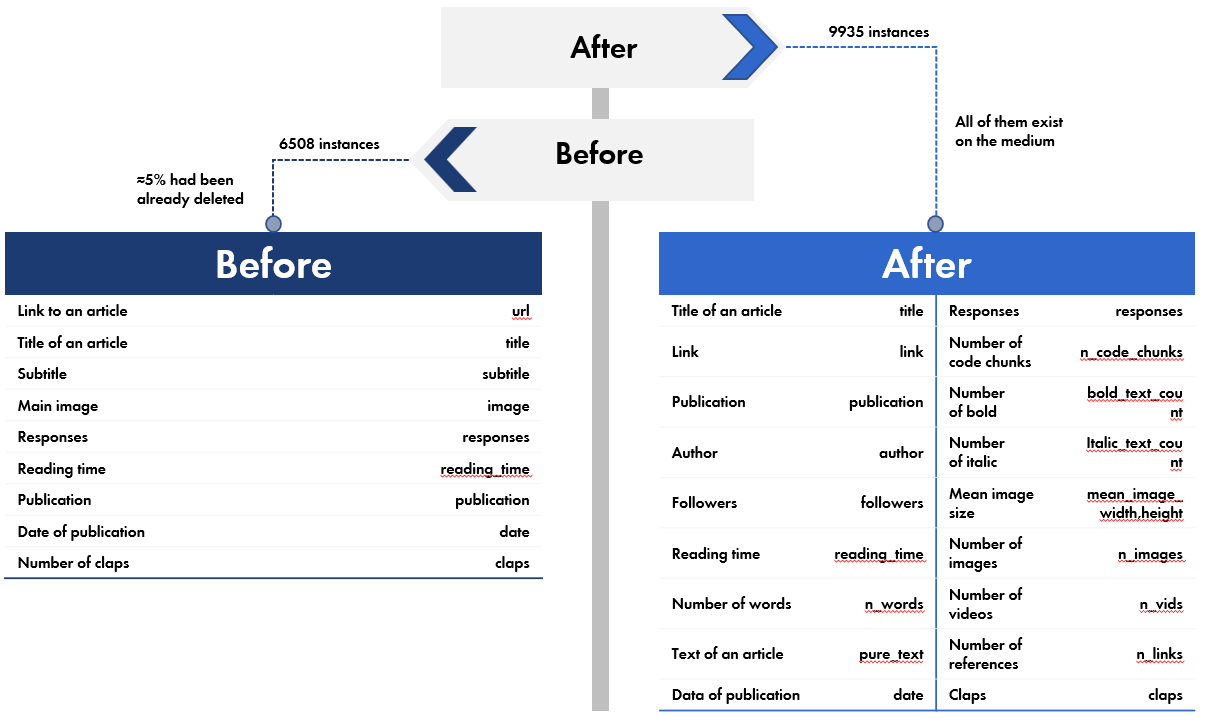
\includegraphics[scale=1]{./scrapping.png}
\end{figure}
\section{EDA and hypothesis testing}
Let's check whether dependencies between claps, length of articles and followers exists or not.
\begin{figure}[H]
    \centering
    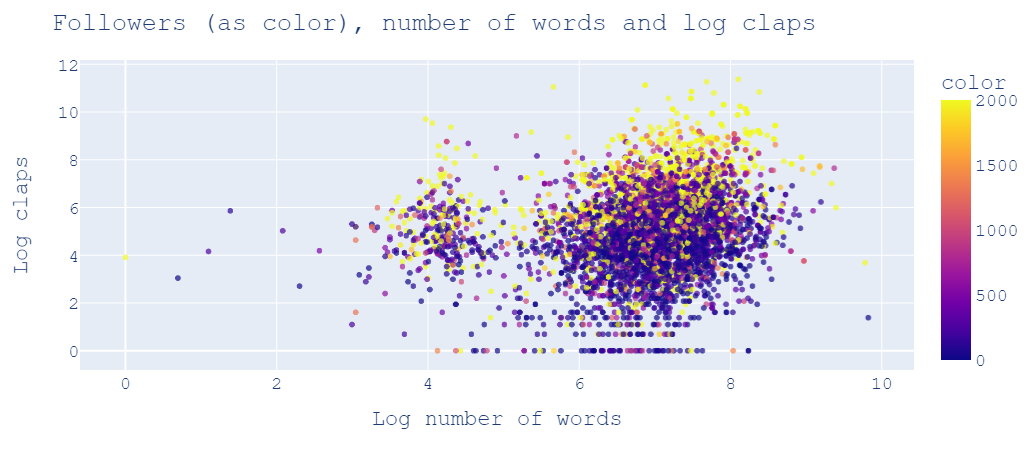
\includegraphics[scale=0.4]{eda1.png}
\end{figure}
As we see, data splits into two clearly separated groups. Moreover, this plot shows that authors with more followers get more claps. However, there is no visible dependency of number of followers and length of articles.
Let's take a look, how publications are located on this plot for 5 most popular publications.
\begin{figure}[H]
    \centering
    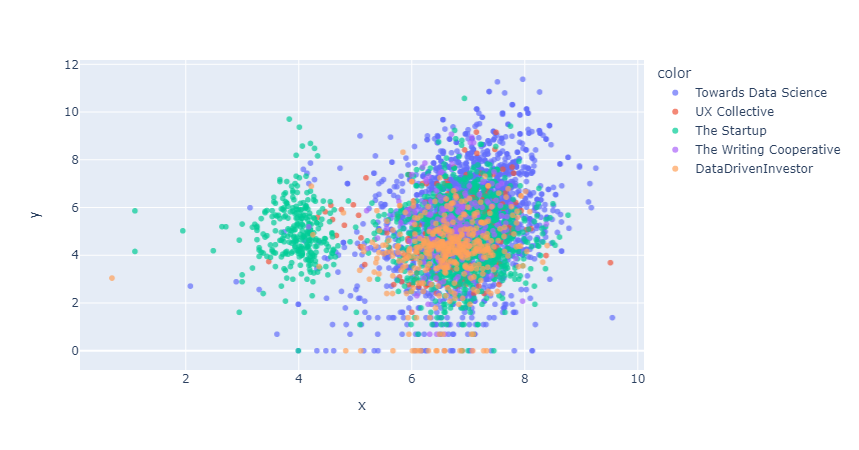
\includegraphics[scale=0.5]{eda2.png}
\end{figure}
The Startup publishings split into two separate groups while others are in the same cluster.
Let's look at 5 most popular topics for The Startup.
\begin{figure}[H]
    \centering
    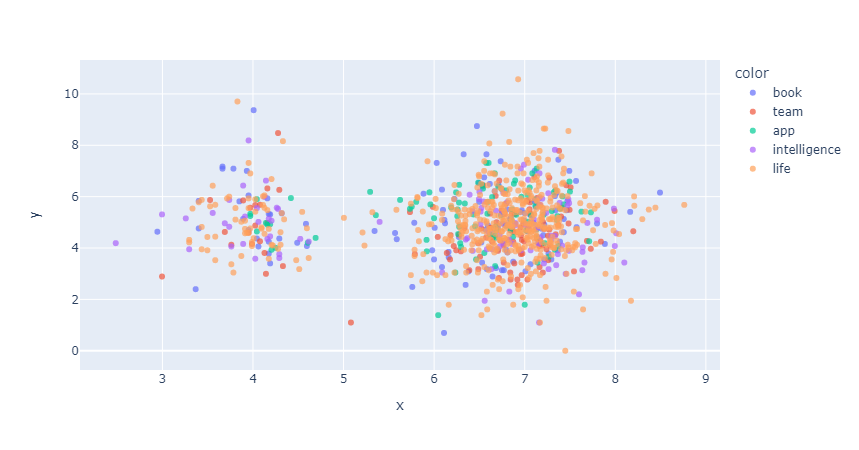
\includegraphics[scale=0.5]{eda3.png}
\end{figure}
There is no visible dependency of cluster and topic of the article.
Let's look at the distribution of claps by 10 most popular topics.
\begin{figure}[H]
    \centering
    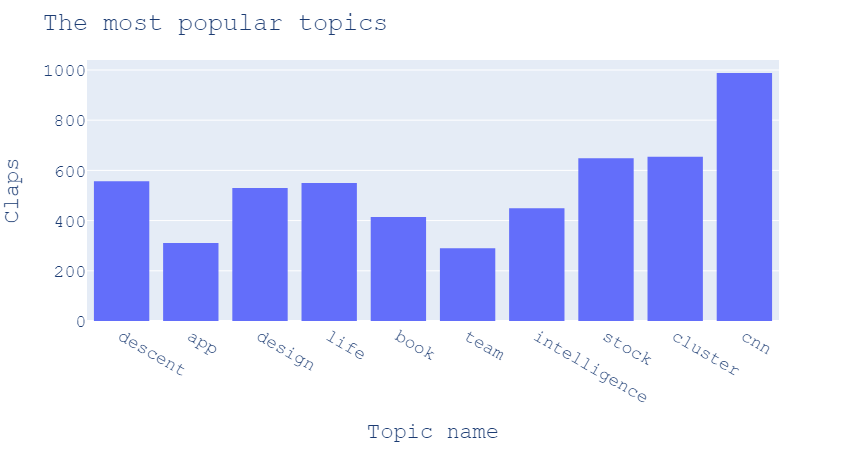
\includegraphics[scale=0.5]{eda4.png}
\end{figure}
As we see "cnn" topic receives the most number of claps between others. Let's check how number of followers relates with of number of claps.
\begin{figure}[H]
    \centering
    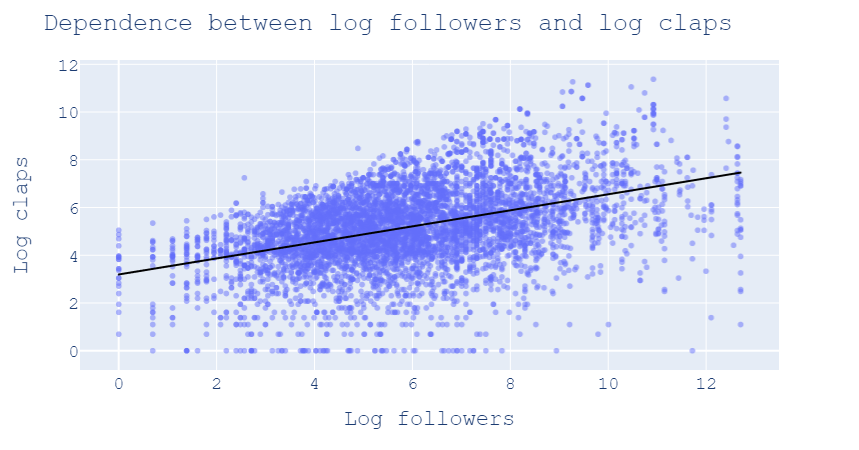
\includegraphics[scale=0.5]{eda5.png}
\end{figure}
Let's check if difference of claps and day of weeks exists.
\begin{figure}[H]
    \centering
    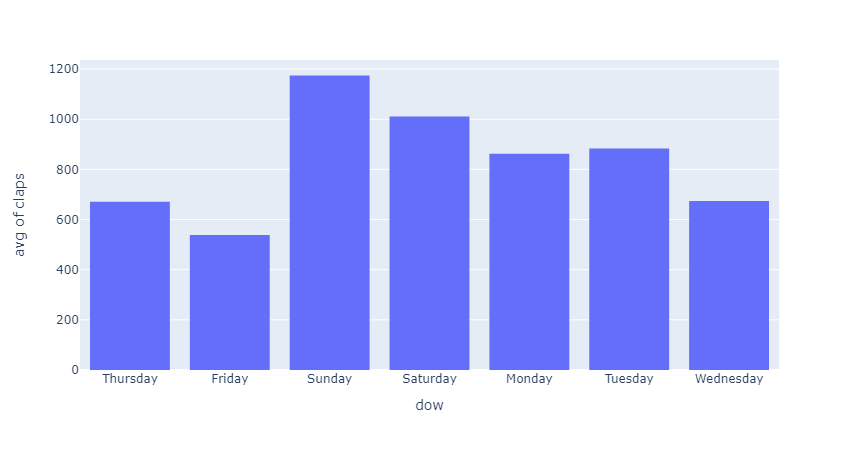
\includegraphics[scale=0.35]{eda6.png}
\end{figure}
I guess the mood on the weekend is better than the work week, so you can put a bunch of claps.
\begin{figure}[H]
    \centering
    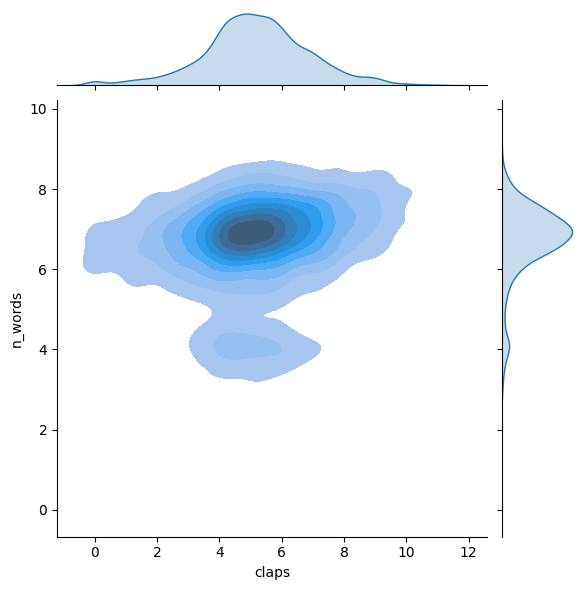
\includegraphics[scale=0.5]{eda7.png}
\end{figure}
Almost no linear dependence.
\begin{figure}[H]
    \centering
    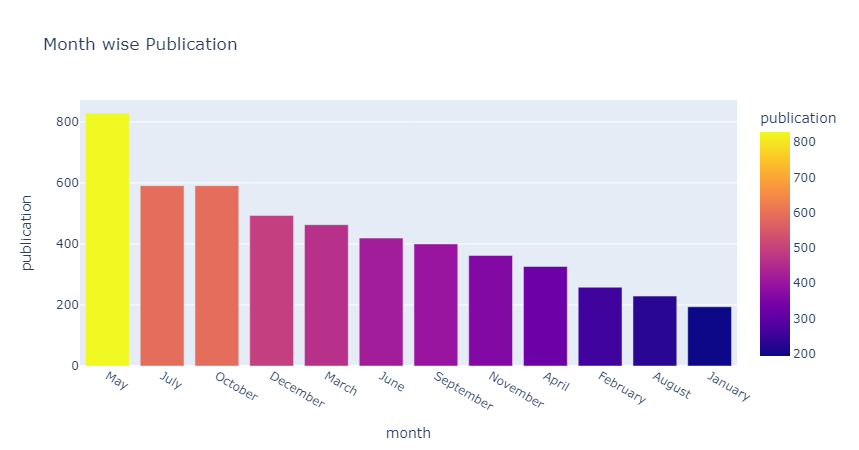
\includegraphics[scale=0.4]{eda8.png}
\end{figure}
The most of publications submitted is in the May. It can be interpreted in the following way: graduation required at the end of the academic year. The least publications submitted in January in case of New Year I suppose.

Let's check equality homoscedasticity and equal of expectations between claps for 3  most popular authors.

Let's check for the normality of the group using the Shapiro-Wilk test:
\[
W =\dfrac{b^2}{s^2},
\]
where $\displaystyle b^2 = \sum\limits_{i=1}^n a_{n-i+1}\left(x_{n-i+1} - x_i\right)$ is the square of Lloyd's standard deviation estimate. Cool. ``p-value'' is significant. Let's first check for homoscedasticity (equality of variances) using the Levene test:
\[
W =\dfrac{N-k}{k-1}\cdot \dfrac{\sum\limits_{i=1}^k N_i\left(Z_{i\cdot} - Z_{\cdot\cdot}\right)^2}{\sum\limits_{i=1}^k\sum\limits_{j=1}^{N_i}N_i\left(Z_{ij} - Z_{i\cdot}\right)},
\]
where $k$ is the number of groups, $N_i$ is the number of study results for the $i$th group, $N$ is the total number of studies, $Y_{ij}$ is the value of the $j$th observation in the $i$th group.
\[
    Z_{ij} = \left|Y_{ij} - \overline{Y}_i\right|,
\]
where $\overline{Y}_i$ is the average of the $i$-th group,
\[
Z_{i\cdot} = \dfrac{1}{N_i}\sum\limits_{j=1}{N_i} Z_{ij},
\]
average of $Z_{ij}$ for the $i$th group,
\[
Z_{\cdot\cdot} = \dfrac{1}{N}\sum\limits_{i=1}^k\sum\limits_{j=1}^{N_i}Z_{ij}
\]
average over all $Z_{ij}$.
\par 
These groups have similar variances. Now we can make a one-way ANOVA test: $p$-value $\approx 0.54 \Rightarrow $ do not reject the hypothesis about expectation equality.

\par 
Let me make the same operations for 10 most popular articles topics. By the $p$-value is close to zero we can obtain that homoscedasticity doesn't save. The same for normaliry. Indeed, only one group is distributed normally, but it's still worth trying \emph{ANOVA-test}.  Let's use \emph{Welch ANOVA}, since it is more robust compared to the classic one. 
\par
We have a low $p$-value, therefore we reject the null hypothesis. After rejecting the null hypothesis, a posteriori Games-Howell test can be performed (it is resistant to homoscedasticity) to determine which group differences are statistically significant. It turns out that the difference between app key word and intelligence is more statistically significant than other pairwise differences.

\par 
Let's try with the articles with low popularity. For homoscedasticity we have good $p$-values, so homoscedasticity is proved. Now let me check whether it normal distributed or not. Only one group is not normal distributed. Let's build \emph{QQ-plot} to see how critical everything is:
\begin{figure}[H]
\centering
  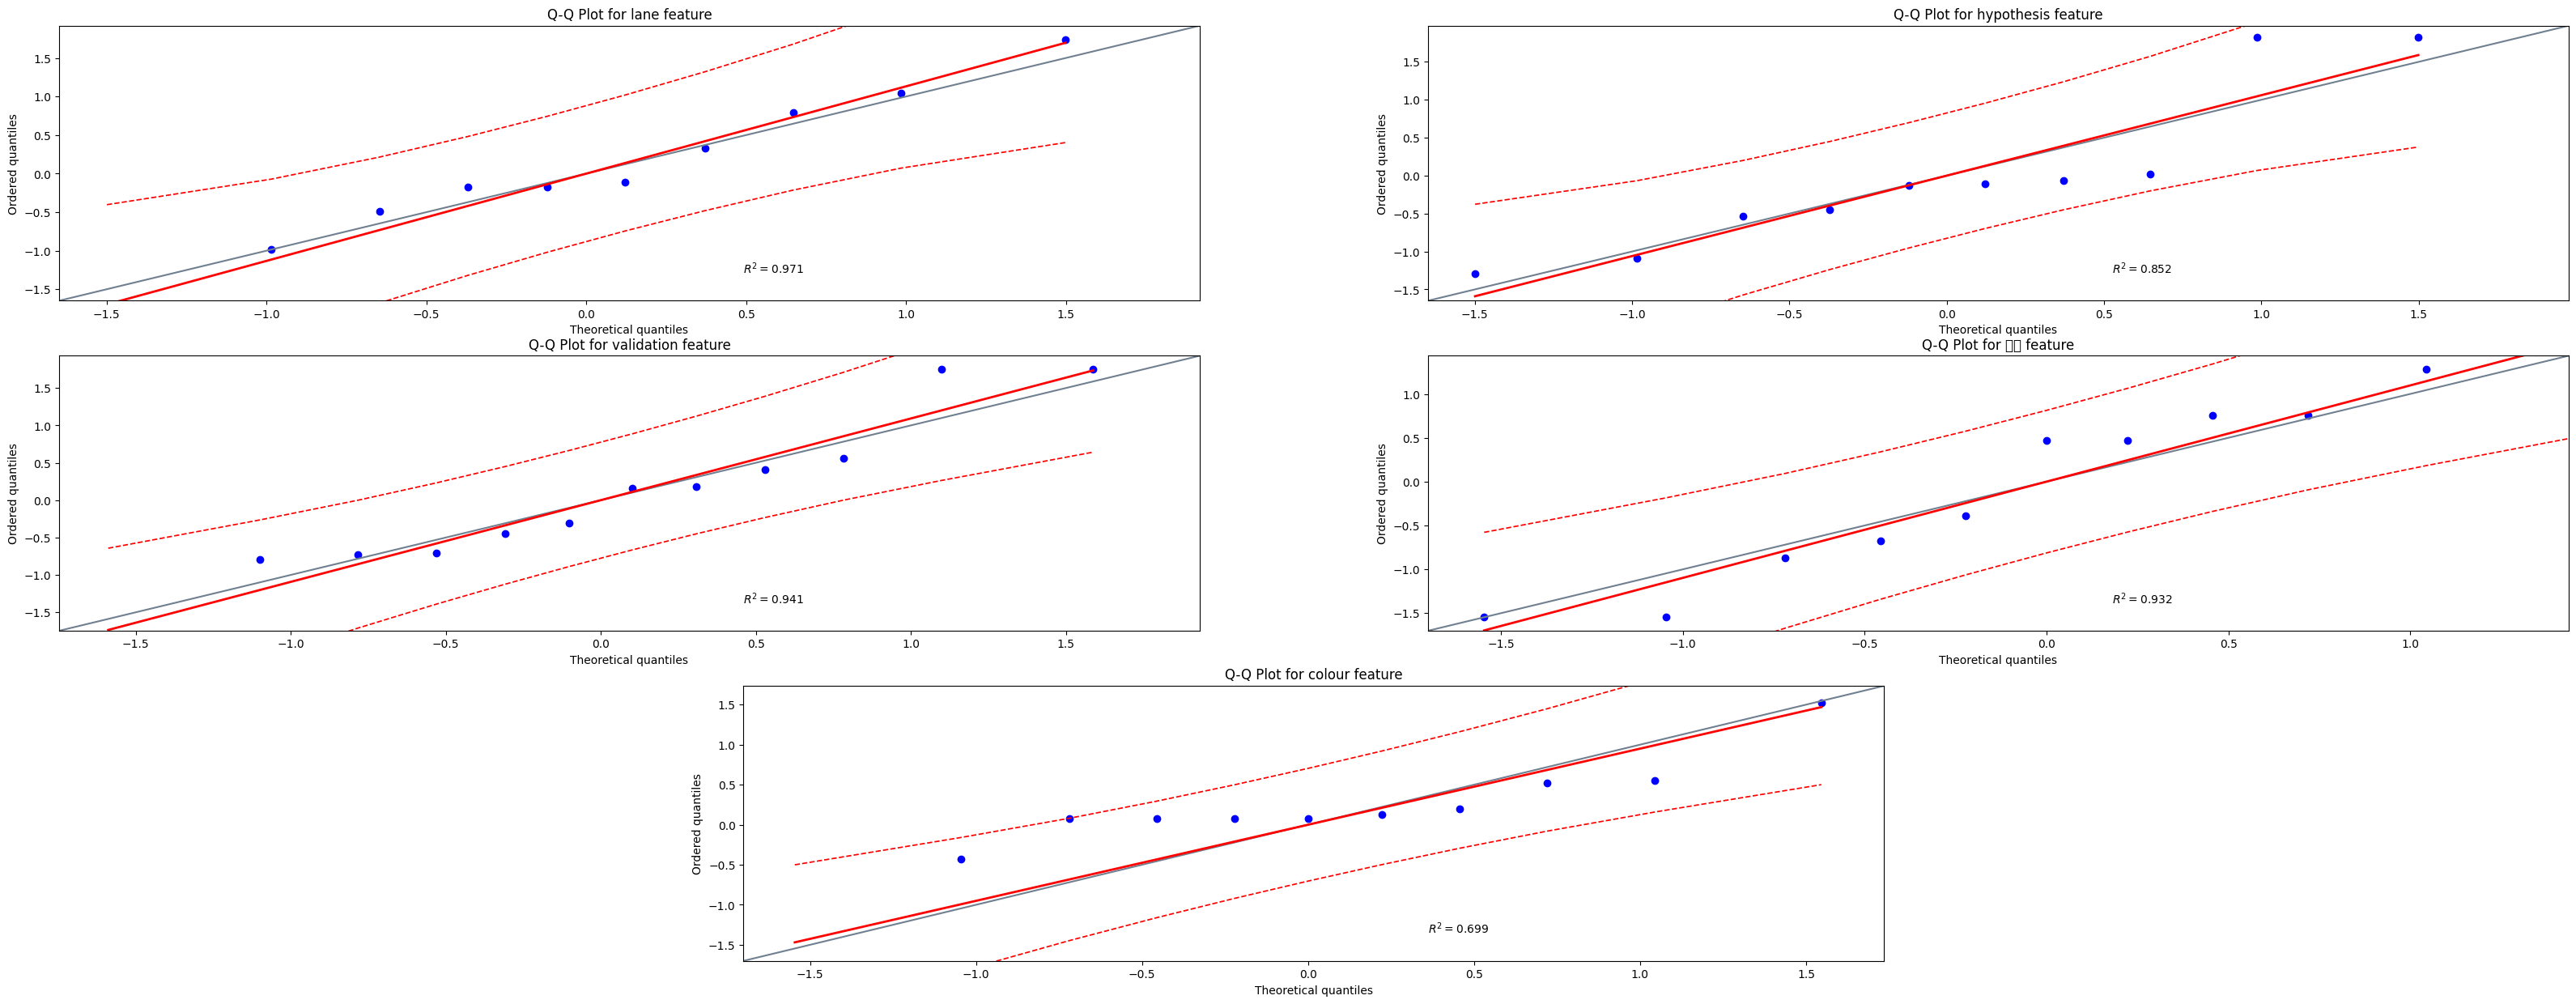
\includegraphics[scale=0.2]{qq.png}
\caption{QQ-plots for by topic names}
\end{figure}
It looks good. Even the worst sample look much more convenient than all objects in the previous iteration. Also ``p-value'' is huge, that is why we cant deny the zero hypothesis.

\section{Topic Modeling}
The task of topic modeling consists in soft clustering of texts on latently contained topics. We formalize the probabilistic formulation of the problem. We will introduce additionally
 $T$ -- a finite set of topics. By the topic we will understand the conditional distribution on a set of terms. Then $P(w|t)$, where $w \in W$ -- word from token set, $t \in T$ -- topic. This conditional probability should be considered as the probability of the term $w$ in topic $t$. Along with this conditional probability, we consider the a posteriori probability necessary to solve the problem $P(t|d)$, meaning the probability of the topic $t\in T$ in text $d \in D$. Thus it is possible to obtain a discrete probability space $D \times W \times T$. As a result, it is necessary to describe the document with a probability distribution of topics $(P(t|d))$, and each topic is a discrete probability distribution of words in the topic $(P(w|t))$. We introduce two hypotheses:
\begin{itemize}
    \item The hypothesis of <<bag of words>>. The word order in the text does not significantly affect the definition of the topic. This allows you to go to the view where $\forall d \in D$  the dictionary of its unique toxins is put in line, the value of the frequency of occurrence of $w$ in the document is calculated and $\forall w \in W$  $d$ $n_{dw}$;
    \item The hypothesis of conditional independence. Tokens in documents depend on the topic, but do not depend on the document. $P(w|t,d) = P(w|t)$.
\end{itemize}
Let 's introduce the notation $P(w|t) = \phi_{wt}$, $P(t|d) = \theta_{td}$. Let's write out the probabilistic distribution of terms in the document with a mixture of previously introduced distributions $P(w|t)$ and $P(t|d)$:
\[P(w|d) = \sum \limits_{t\in T} P(w|t)P(t|d) = \sum\limits_{t\in T} \phi_{wt}\theta_{td}.\]
In finding matrices $\Phi = \left(\phi_{wt}\right)_{\dim{W}\times \dim{T}}$ and $\Theta = \left(\theta_{td}\right)_{\dim{T} \times \dim{D}}$ and the task of mathematical modeling is. This problem can also be described through the stochastic matrix decomposition heuristic (Figure \ref{fig:svd}).
\begin{figure}[H]
    \centering
    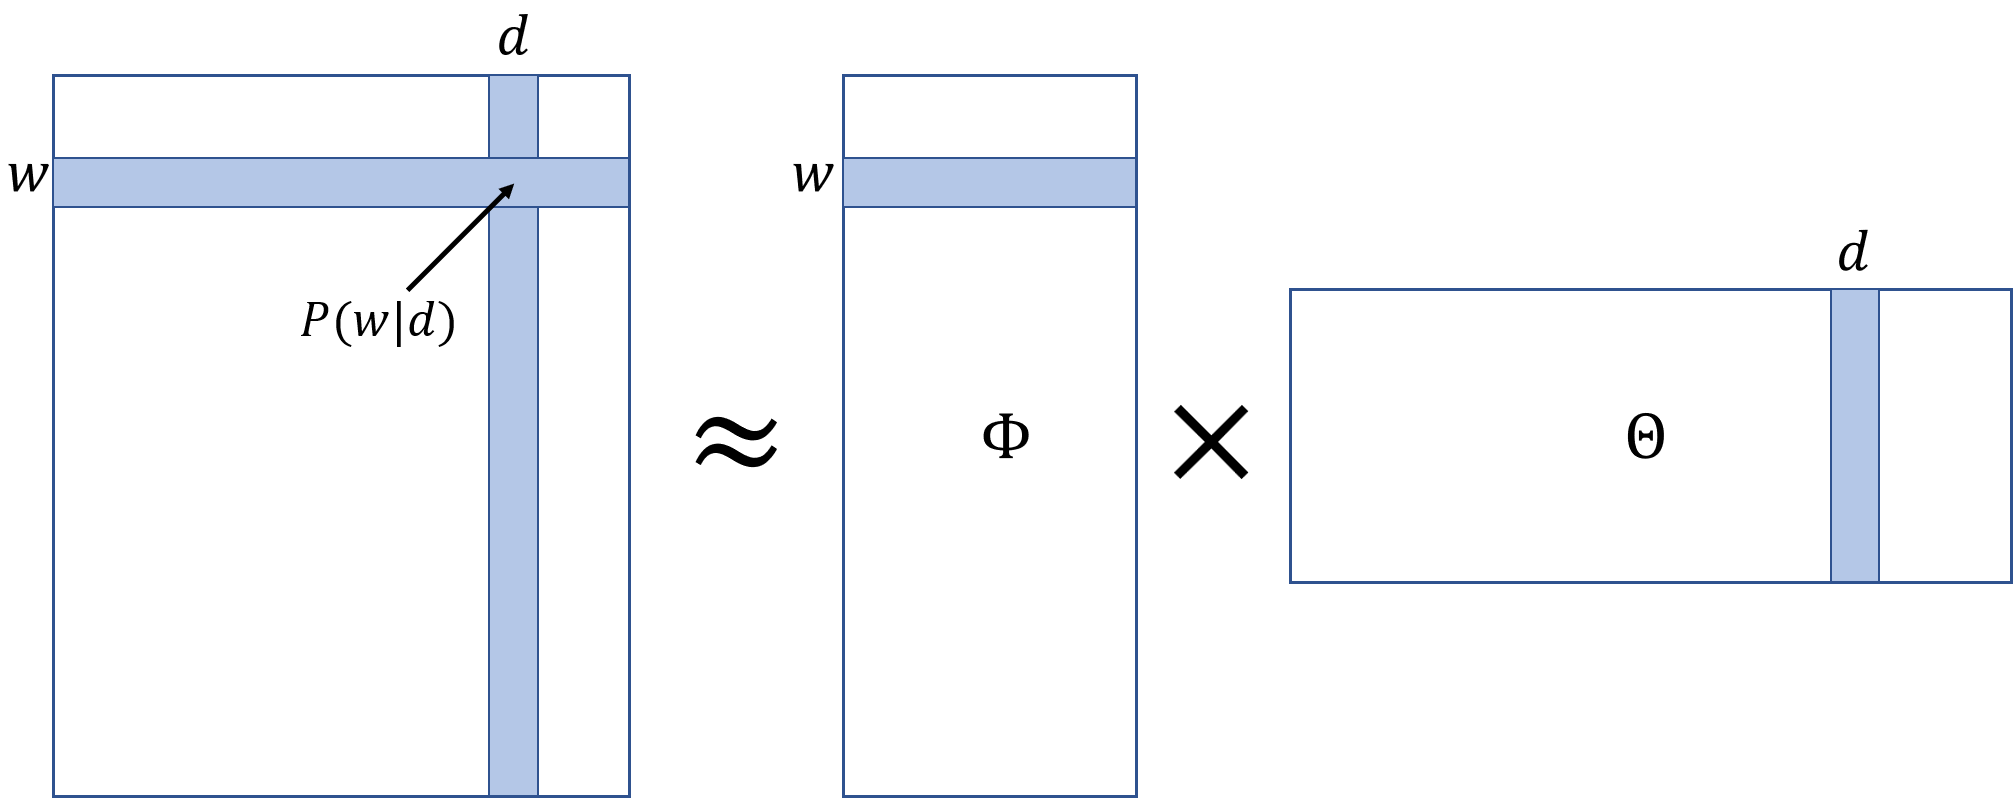
\includegraphics[scale=0.5]{./svd.png}
    \caption{Stochastic matrix factorization}
    \label{fig:svd}
\end{figure}

Let's write down the density of the sample distribution $\left(d_i, w_i\right)_{i=1}^{n}$:
\[\prod_{i=1}^{n} p(d_i, w_i) = \prod_{d\in D} \prod_{w\in d} p(d,w)^{n_{dw}},\]
which is essentially a likelihood function. Then the maximization of the logarithm of likelihood will be written as:
\[\sum\limits_{d\in D}\sum\limits_{w\in d} n_{dw} \ln p(w|d)p(d) \to \max_{\Phi, \Theta}.\]
We have a mathematical programming problem:
\[\sum\limits_{d\in D}\sum\limits_{w\in d} n_{dw} \ln\sum\limits_{t\in T} \phi_{wt}\theta_{td}\to \max_{\Phi, \Theta}\]
with the limitations of non-negativity and normalization imposed by Kolmogorov's axiomatics:
\[\phi_{wt} \geq 0, \hspace*{0.3cm} \sum\limits_{w\in W} \phi_{wt} = 1; \hspace*{0.5cm} \theta_{td} \geq 0, \hspace*{0.3cm} \sum\limits_{t\in T} \theta_{td} = 1.\]
Due to the lack of a correct Hadamard formulation of the problem, it is necessary to apply regularization
%! write about the non-uniqueness of the solution
Maximizing the likelihood logarithm with ARTM regularization:
\[\sum\limits_{d,w} n_{dw} \ln \sum\limits_{t\in T} \phi_{wt}\theta_{td} + R(\Phi, \Theta) \to \max_{\Phi, \Theta}, \hspace*{0.3cm} R(\Phi, \Theta) = \sum\limits_{i} \tau_i R_i(\Phi, \Theta).\]
EM-algorithm.
\bigskip\par
E-step:
\[p_{tdw} = p(t|d,w) = \underset{t\in T}{\text{norm}}\left(\phi_{wt}\theta_{td}\right)\]
M-step:
\[\phi_{wt} = \underset{w\in W}{\text{norm}} \left(n_{wt} + \phi_{wt}\dfrac{\partial R}{\partial \phi_{wt}}\right), \hspace*{0.3cm} n_{wt} = \sum\limits_{d\in D}n_{dw}p_{tdw}\]
\[\theta_{td} = \underset{t\in T}{\text{norm}} \left(n_{td} + \theta_{td} \dfrac{\partial R}{\partial \theta_{td}}\right), \hspace*{0.3cm} n_{td} = \sum\limits_{w\in d} n_{dw} p_{tdw},\]
where $\underset{x\in X}{\text{norm}} (y_x) =\dfrac{\max\left\{y_x, 0\right\}}{\sum\limits_{k\in X}\max\left\{x_k,0\right\}}$
E-step: conditional probabilities of $p(t|d, w)$ are calculated using a posteriori probabilities $\phi_{wt}, \\theta_{td}$ by Bayes formula:
\[p(t|d,w) = \dfrac{p(w,t|d)}{p(w|d)} = \dfrac{p(w|t)p(t|d)}{p(w|d)} = \dfrac{\phi_{wt}\theta_{td}}{\sum\limits_{k}\phi_{wk}\theta_{kd}}.\]
M-step: at $R = 0$, the frequency characteristics are calculated by summing $n_{tdw} = n_{dw} p(t|d, w)$:
\[\phi_{wt} = \dfrac{n_{wt}}{n_t}, \hspace*{0.3cm} n_{wt} = \sum\limits_{d\in D} n_{tdw}, \hspace*{0.3cm} n_t = \sum\limits_{w\in W} n_{wt}\]
\[\theta_{td} = \dfrac{n_{td}}{n_d}, \hspace*{0.3cm} n_{td} = \sum\limits_{w\in d} n_{tdw}, \hspace*{0.3cm} n_d = \sum\limits_{t\in T} n_{td}.\]
For pLSA:
\[R(\Phi, \Theta) = 0.\]
M-step -- frequency estimates of conditional probabilities:
\[\phi_{wt} = \underset{w\in W}{\text{norm}}(n_{wt}), \hspace*{0.3cm} \theta_{td} = \underset{t\in T}{\text{norm}}(n_{td}).\]
\subsubsection{Latent Dirichlet Placement (LDA)}
Regularization:
\[R(\Phi, \Theta) = \sum\limits_{t,w} \left(\beta_w - 1\right)\ln \phi_{wt} + \sum\limits_{d,t} \left(\alpha_t - 1\right) \ln\theta_{td}.\]
M-step -- smoothed frequency characteristics with parameters $\beta_w, \alpha_t$:
\[\phi_{wt} = \underset{w\in W}{\text{norm}}(n_{wt} + \beta_w - 1), \hspace*{0.3cm} \theta_{td} = \underset{t\in T}{\text{norm}}(n_{td} + \alpha_t - 1).\]
\textbf{Hypothesis}: Vectors $\phi_t = \left(\phi_{wt}\right)$ and $\theta_d = \left(\theta_{td}\right)$ are generated by Dirichlet distributions, with $\alpha\in \mathbb{R}^{|T|}, \\beta\in\mathbb{R}^{|W|}:$
\[\text{$Dir(\phi_t|\beta)$} = \dfrac{\Gamma(\beta_0)}{\prod_{w\in W}\Gamma (\beta_w)} \prod_{w\in W} \phi_{wt}^{\beta_w-1}, \hspace*{0.3cm} \phi_{wt} > 0; \hspace*{0.3cm} \beta_0 = \sum\limits_{w \in W} \beta_w, \ \beta_t > 0;\]
\[\text{$Dir(\theta_d| \alpha)$} = \dfrac{\Gamma(\alpha_0)}{\prod_{t\in T}\Gamma (\alpha_t)} \prod_{t\in T} \theta_{td}^{\alpha_t-1}, \hspace*{0.3cm} \theta_{td} > 0; \hspace*{0.3cm} \alpha_0 = \sum\limits_{t \in T} \alpha_t, \ \alpha_t > 0;\]
Let's write down the a posteriori probability for LDA:
\[\ln \prod_{d\in D} \prod_{w\in d} p(w,d | \Phi, \Theta)^{n_{dw}} = \prod_{t \in T}\text{Dir}(\phi_t| \beta) \prod_{d\in D} \text{Dir}(\theta_d|\alpha) \to \max_{\Phi, \Theta}\]
\begin{itemize}
\item when $\beta_w > 1, \\alpha_t > 1$ -- smoothing;
\item at $\beta\in (0,1), \\alpha\in (0,1)$ -- weak dilution,
\item at $\beta = \alpha = 1$ -- pLSA.
\end{itemize}

\subsubsection{BERT Topic}
Another approach to solving the problem of thematic modeling is clustering in the vector space of texts with neural network vectorization of texts. One of the most relevant models in solving this problem is BERTopic. Stages of the algorithm operation:
\begin{enumerate}
\item Text vectorization (pre-trained models of Bert Embeddings );
\item Dimension reduction (by UMAP method);
During operation, the algorithm builds a weighted graph, connecting only those vertices that are the nearest neighbors. Let $X\in\mathbb{R}^n$ be the vertices of a graph (a vector of words in $n$-dimensional space). $T\in\mathbb{R}^{k}$ -- the set of $k$-closest to $x_i\\forall i$. For each object, the distance to the nearest neighbor and the value of $\sigma_i$ are calculated according to the formulas, respectively:
\[\rho_i = \min\limits_{t\in T} d(x_i, t),\]
\[\sum\limits_{i}e^{-\left(\dfrac{d(x_i,y) - \rho_i}{\sigma_i}\right)} = \log_2 k\]
The weight of the edge connecting $x_i$ and its neighbor $t_k$ is determined by the formula:
\[w_{ij} = e^{-\left(\dfrac{d(x_i, t_j) -\rho_i}{\sigma_i}\right)}.\]
The set of edges of the constructed graph is fuzzy with the probability of the existence of an edge between two vertices as a function of membership. The weight of an edge between two vertices is determined by the formula:
\[w_{x_i, x_j} = w(x_j \to x_i) + w(x_i \to x_j) - w(x_i \to x_j) \cdot w(x_j\to x_i).\]
Then the graph is constructed in a low-dimensional space and approximated with the original by minimizing the sum of the Kullback-Leibler divergences for each of the edges $e$ from the original and new fuzzy sets:
\[\sum\limits_{e\in E} w_h(e)\log\dfrac{w_h(e)}{w_l(e)} + (1-w_h(e))\log\left(\dfrac{1-w_h(e)}{1-w_l(e)}\right) \to \min\limits_{w_l},\]
$w_h(e)$ is the membership function of a fuzzy set of edges in a high-dimensional space, $w_l(e)$ is the membership function of a fuzzy set of edges in a low-dimensional space. The optimization problem is solved using stochastic gradient descent.
\item Clustering (HDBSCAN method) :
\begin{figure}
\centering
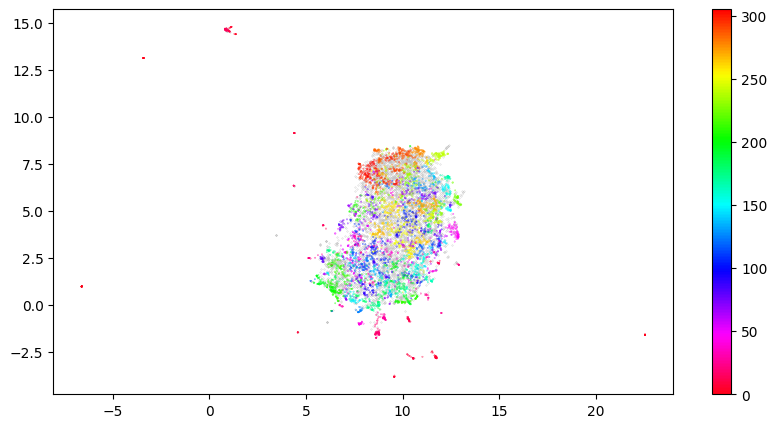
\includegraphics[scale=0.75]{hdbscan.png}
\caption{The result of HDBSCAN for our dataset}
\label{fig:hdbscan}
\end{figure}
\end{enumerate}
Formalize HDBSCAN.
\begin{enumerate}
\item Let $U_\epsilon(x)$ -- $\epsilon$ be the neighborhood of the point $x$ that has not been viewed before.
\item If a point $x$ contains $minPts$ neighbors (where $minPts$ and the metric by which the distance between the points is located are the specified hyperparameters) or more, then a cluster is formed
\item Otherwise the point is marked with noise. We return to item 1.
\item Repeat, item 2-3 until a connected cluster is obtained (there is at least one path between any neighbors);
\item Repeat steps 1-4 for a new point that has not been viewed.
\end{enumerate}
\begin{figure}[H]
    \centering
    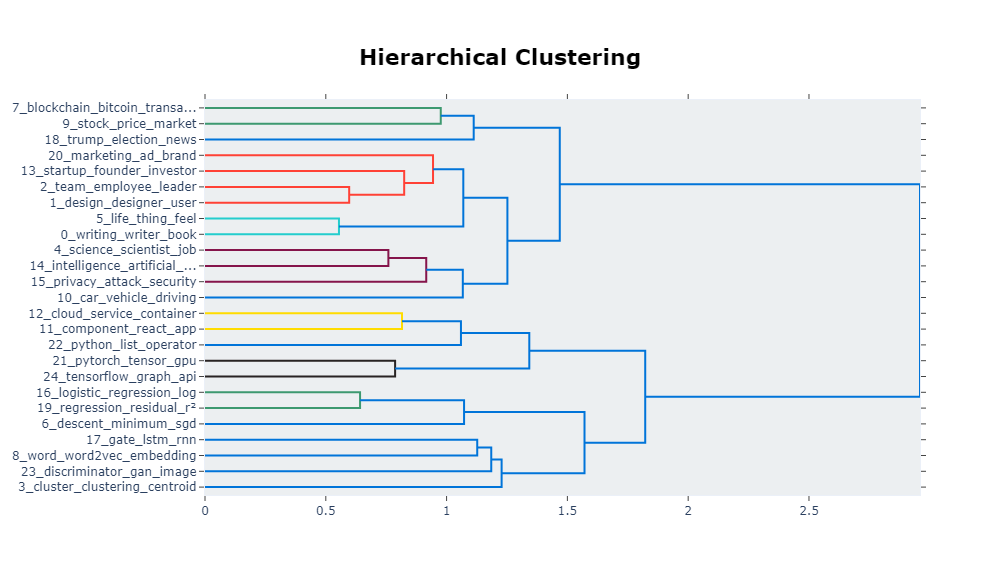
\includegraphics[scale=0.4]{hierarchy.png}
\end{figure}
\begin{figure}[H]
    \centering
    
\includegraphics[scale=0.4]{topic.png}
    
\includegraphics[scale=0.4]{topic1.png}
    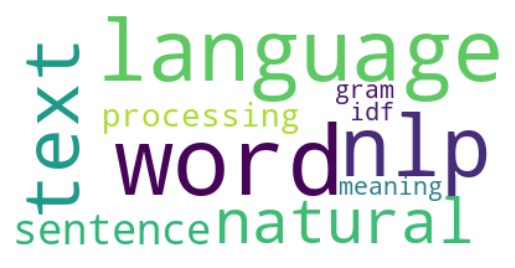
\includegraphics[scale=0.4]{topic2.png}
    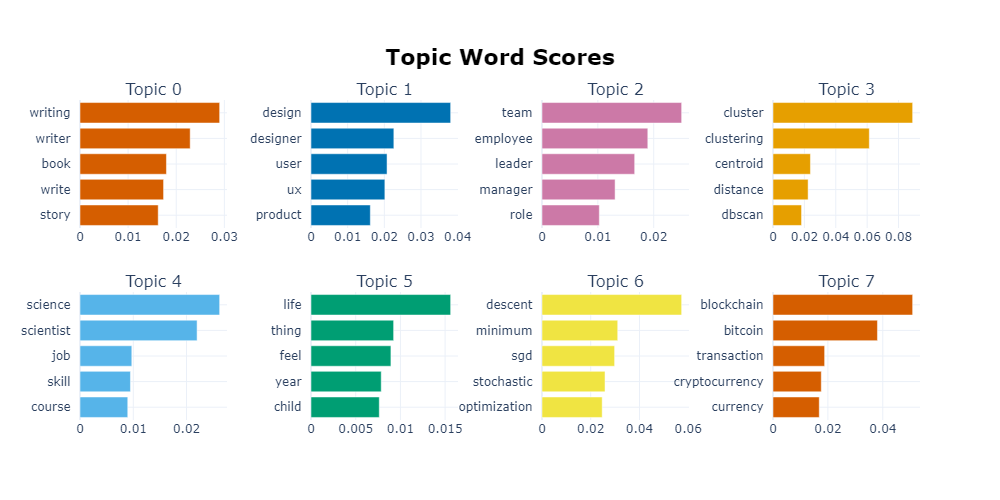
\includegraphics[scale=0.4]{topic_score.png}
\end{figure}
\begin{figure}[H]
    \centering
    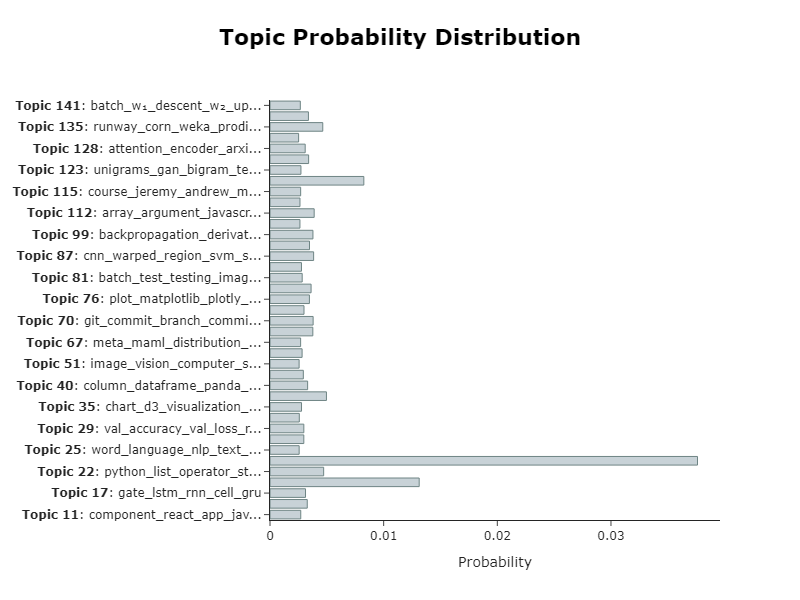
\includegraphics[scale=0.5]{topic_distribution.png} 
\end{figure}
\section{Regression}
The main idea was to build the state-of-the-art boostings: Catboost, XGboost, LightGBM. Then build an ensembling on them according to the principle
\[ res = x_1 cat\_boost + x_2 xgboost + (1-x_1-x_2) lightgbm\]
and obtain by optuna the optimal values of $x_1, x_2$. 
\begin{table}[H]
    \centering
    \begin{tabular}{|l|l|l|l|}
    \hline
    optuna & catboost & xgboost & lightgbm \\ \hline
    282.2  & 307.4    & 297.3   & 353      \\ \hline
    \end{tabular}
    \end{table}
\section{Error analysis}
Lets evaluate our model through cross-validation, obtain estimators from every step, get predictions from it, compute residuals and compare them in homoscedasticity sense. It will mean that our model saves homoscedasticity through cross-validation, it is stable and working well. In this case I have trained on log claps, not merely claps. I perfomed Levene test and obtained, that our model is stable.
\begin{figure}[H]
    \centering
    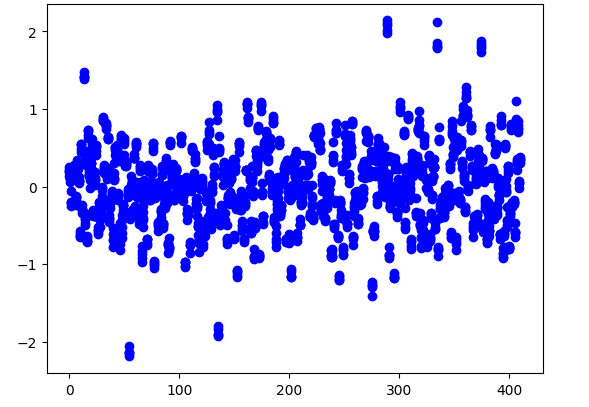
\includegraphics[scale=0.5]{residuals.png} 
\end{figure} 
\newpage
{\Large ToDo list}:
\begin{todolist}
  \item Check the biggest errors and analyze it;
  \item Try to get rid off outliers;
  \item Perfom it without outliers and compare the results;
  \item Feature importances (Random forest, Recursive Feature Elimination);
  \item Dimension reduction.
\end{todolist}
\end{document}
